\documentclass{standalone}

\usepackage{tikz}

\begin{document}
  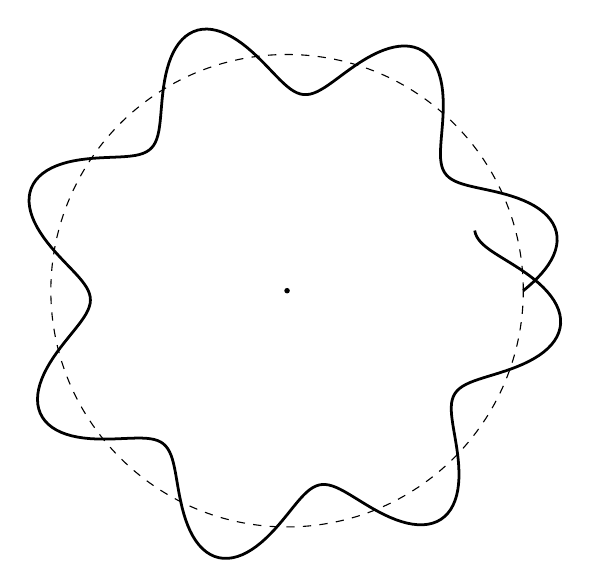
\begin{tikzpicture}
    \coordinate (O) at (0,0);
    \fill (O) circle (1pt);
    \draw[dashed] (O) circle (3);
    \draw[domain=0:2.1*pi,samples=400,line width=1pt]
      plot ({deg(\x)}:{3+0.5*sin(deg(7.4*\x))});
  \end{tikzpicture}

  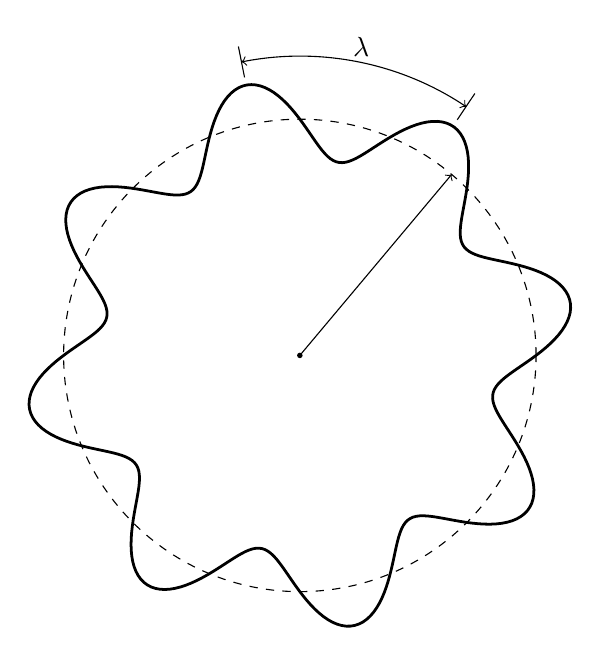
\begin{tikzpicture}
    \coordinate (O) at (0,0);
    \fill (O) circle (1pt);
    \draw[dashed] (O) circle (3);
    \draw[domain=0:2*pi,samples=400,line width=1pt]
      plot ({deg(\x)}:{3+0.5*sin(deg(8*\x))});

    \draw (56.25:3.6) --+ (56.25:0.4) (101.25:3.6) --+ (101.25:0.4);
    \draw[<->] (56.25:3.8) arc (56.25:101.25:3.8);
    \node at (78.75:4){$\lambda$};
    \draw[->] (O) -- (50:3);
  \end{tikzpicture}
\end{document}
